\documentclass{exam}
\usepackage{commonheader}
\usepackage{hyperref}

%%% CHANGE THESE %%%%%%%%%%%%%%%%%%%%%%%%%%%%%%%%%%%%%%%%%%%%%%%%%%%%%%%%%%%%%%
\discnumber{10}
\title{\textsc{Final Review}}
\date{April 24 to April 26, 2017}
%%%%%%%%%%%%%%%%%%%%%%%%%%%%%%%%%%%%%%%%%%%%%%%%%%%%%%%%%%%%%%%%%%%%%%%%%%%%%%%

\begin{document}
\maketitle
\rule{\textwidth}{0.15em}
\fontsize{12}{15}\selectfont

%%% INCLUDE TOPICS HERE %%%%%%%%%%%%%%%%%%%%%%%%%%%%%%%%%%%%%%%%%%%%%%%%%%%%%%%

\section{What Would Python Print? Iterators}
\begin{questions}

\begin{blocksection}
\question
\begin{lstlisting}
class SkipIterator:
    def __init__(self, rng, n):
        self.obj = rng
        self.skip = n

    def __iter__(self):
        return self

    def __next__(self):
        result = self.obj.curr
        self.obj.curr += self.skip
        return result

class SkippedNaturals:
    def __init__(self):
        self.curr = 0
        self.skip = 1

    def __iter__(self):
        return SkipIterator(self, self.skip)
\end{lstlisting}
\end{blocksection}

\begin{blocksection}
\begin{tabular}{|l|l|}
\hline
\textbf{Expression} & \textbf{Interactive Output}\\\hline
\begin{lstlisting}
p = SkippedNaturals()
twos = iter(p)
p.skip = p.skip + 1
threes = iter(p)
next(twos)
\end{lstlisting}
& \\\hline
\begin{lstlisting}
next(twos)
\end{lstlisting}
& \\\hline
\begin{lstlisting}
next(threes)
\end{lstlisting}
& \\\hline
\begin{lstlisting}
next(threes)
\end{lstlisting}
& \\\hline
\end{tabular}

\begin{solution}
\begin{tabular}{|c|}
\hline
0\\\hline
1\\\hline
2\\\hline
4\\\hline
\end{tabular}
\end{solution}

\end{blocksection}

\section{Environment Diagrams}

\begin{blocksection}
\question Draw the environment diagram for the following code snippet:
\begin{lstlisting}
def one(two):
    three = two
    def four(five):
        nonlocal three
        if len(three) < 1:
            three.append(five)
            five = lambda x: four(x)
        else:
            five = seven + 7
        return five
    two = two + [1]
    seven = 8
    return four(three)

eight = one([])
print(eight(9))
\end{lstlisting}
\end{blocksection}

\begin{solution}
\url{https://goo.gl/d71WTd}
\linebreak
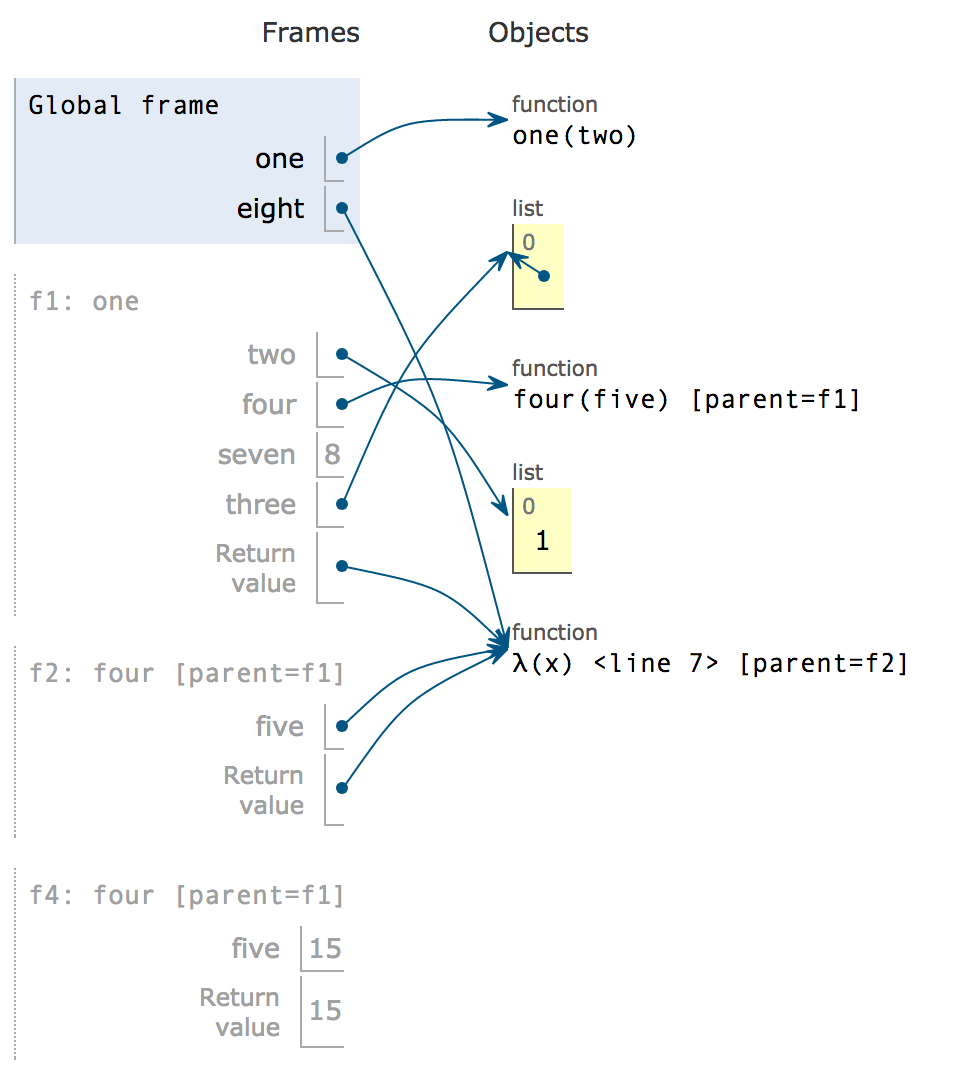
\includegraphics[width=0.85\textwidth]{envdiag}

\end{solution}

\section{Recursive Data Structures}

\begin{blocksection}
\question DoubleTree hired you to architect one of their hotel expansions!  As
you might expect, their floor plan can be modeled as a tree and the expansion
plan requires doubling each node (the patented double tree floor plan). Here's
what some sample expansions look like:\\\\
\begin{tabular}{c c}
\textbf{Before} & \textbf{After}\\
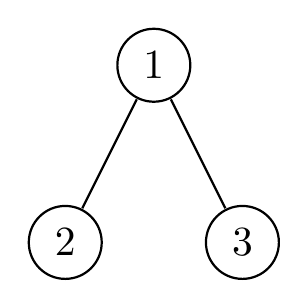
\begin{tikzpicture}[thick, scale=1.5, transform shape]
    \node [circle, draw] (z){$1$}
        child {node [circle, draw] (a) {$2$}}
        child {node [circle, draw] (b) {$3$}}
        ;
\end{tikzpicture}
&
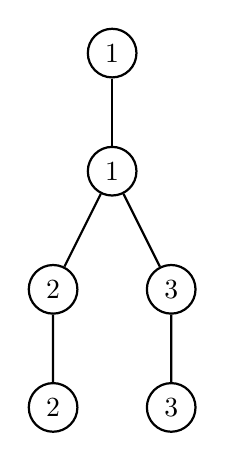
\begin{tikzpicture}[thick, scale=1.0, transform shape]
    \node [circle, draw] (z){$1$}
        child {node [circle, draw] (a) {$1$}
            child {node [circle, draw] (b) {$2$}
                child {node [circle, draw] (d) {$2$}}
            }
            child {node [circle, draw] (c) {$3$}
                child {node [circle, draw] (e) {$3$}}
            }
        }
        ;
\end{tikzpicture}
\end{tabular}

Fill in the implementation for \texttt{double\char`_tree}.

\begin{lstlisting}
def double_tree(t):
    """
    Given a tree, return a new tree where entries appear
    twice.
    >>> double_tree(Tree(1))
    Tree(1, [Tree(1)])
    >>> double_tree(Tree(1, [Tree(2), Tree(3)]))
    Tree(1, [Tree(1, [Tree(2, [Tree(2)]),
                      Tree(3, [Tree(3)])
                     ])
            ])
    """
\end{lstlisting}
\begin{solution}[0.5in]
\begin{lstlisting}
    if t.is_leaf():
        return Tree(t.label, [Tree(t.label)])
    else:
        dbl_branches = [double_tree(c) for c in t.branches]
            return Tree(t.label,
                        [Tree(t.label, dbl_branches)])
\end{lstlisting}
\end{solution}
\end{blocksection}

\begin{blocksection}
\question Fill in the implementation of \texttt{double\char`_link}.

\begin{lstlisting}
def double_link(lst):
    """
    Using mutation, replaces the second in each pair of items
    with the first. The first of each pair stays as is.
    >>> double_link(Link(1, Link(2, Link(3, Link(4)))))
    Link(1, Link(1, Link(3, Link(3))))
    >>> double_link(
            Link('c', Link('s', Link(6, Link(1, Link('a')))))
        )
    Link('c', Link('c', Link(6, Link(6, Link('a')))))
    """
    if __________________________________________:
        return __________________________________
    _____________________________________________
    _____________________________________________
    return ______________________________________
\end{lstlisting}
\begin{solution}[0.5in]
\begin{lstlisting}
    if lst is Link.empty or lst.rest is Link.empty:
        return lst
    lst.rest.first = lst.first
    double_link(lst.rest.rest)
    return lst
\end{lstlisting}
\end{solution}
\end{blocksection}

\begin{blocksection}
\question Fill in the implementation of \texttt{shuffle}.

\begin{lstlisting}
def shuffle(lst):
    """
    Swaps each pair of items in a linked list.
    >>> shuffle(Link(1, Link(2, Link(3, Link(4)))))
    Link(2, Link(1, Link(4, Link(3))))
    >>> shuffle(
            Link('s', Link('c', Link(1, Link(6, Link('a')))))
        )
    Link('c', Link('s', Link(6, Link(1, Link('a')))))
    """
    if _________________________________________________
        return _______________________________________
    new_head = lst.rest
    lst.rest = _________________________________________
    ____________________________________________________
    return _____________________________________________
\end{lstlisting}

\begin{solution}[0.5in]
\begin{lstlisting}
    if lst == Link.empty or lst.rest == Link.empty:
        return lst
    new_head = lst.rest
    lst.rest = shuffle(new_head.rest)
    new_head.rest = lst
    return new_head
\end{lstlisting}
\end{solution}
\end{blocksection}

\section{Scheme}

\begin{blocksection}
\question Write a Scheme function insert that creates a new list that would
result from inserting an item into an existing list at the given index. Assume
that the given index is between 0 and the length of the original list,
inclusive.

\begin{lstlisting}[language=Scheme]
(define (insert lst item index)



)
\end{lstlisting}

\begin{solution}
\begin{lstlisting}[language=Scheme]
(define (insert lst item index)
  (if (= index 0)
    (cons item lst)
    (cons (car lst) (insert (cdr lst) item (- index 1))))
)
\end{lstlisting}
\end{solution}

\textbf{Extra:} Write this as a tail recursive function. Assume append is tail
recursive.
\begin{solution}
\begin{lstlisting}[language=Scheme]
(define (insert lst item index)
  (define (helper lst index so-far)
    (if (or (null? lst) (= index 0))
      (append so-far (cons item lst))
      (helper (cdr lst) (- index 1)
              (append so-far (list (car lst))))
    )
  )
  (helper lst index nil)
)
\end{lstlisting}
\end{solution}
\end{blocksection}

\section{Interpreters}
\begin{blocksection}
\question Circle the number of calls to \texttt{scheme\char`_eval} and
\texttt{scheme\char`_apply} for the code below.

\begin{lstlisting}[language=Scheme]
(define (square x) (* x x))
(+ (square 3) (- 3 2))
\end{lstlisting}

\begin{tabular}{l | r r r r}
    Calls to \texttt{scheme\char`_eval} (circle one) & 2 & 5 & 14 & 24\\
    \hline
    Calls to \texttt{scheme\char`_apply} (circle one) & 1 & 2 & 3 & 4
\end{tabular}
\begin{solution}
14 for eval, 4 for apply.
\end{solution}
\end{blocksection}

\section{Recursive Select in SQL}
\begin{blocksection}
\question Create a \texttt{mod\char`_seven} table that has two columns, a number
from 0 to 100 and then its value mod 7.\\
\textbf{Hint:} You can create a table first with all of the initial data you
will build from, and then build the \texttt{mod\char`_seven} table.

\begin{solution}[1in]
\begin{lstlisting}[language=SQL]
with
    base(n) as (
        select 0 union
        select n+1 from base where n+1<7
    ),
    mod_seven (n, value) as (
        select n, n from base union
        select n+7, value from mod_seven where n+7<=100
    )
select * from mod_seven;

ALTERNATIVE SOLUTION WITH MODULO OPERATOR
with
    mod_seven (n, value) as (
        select 0, 0 union
        select n+1, (n+1)%7 from mod_seven where n<100
     )
select * from mod_seven;

ALTERNATIVE SOLUTION WITH ONE TABLE
(This could be a pre-step to approaching the original solution.)
with
    mod_seven (n, value) as (
        select 0, 0 union
        select 1, 1 union
        select 2, 2 union
        select 3, 3 union
        select 4, 4 union
        select 5, 5 union
        select 6, 6 union
        select n+7, value from mod_seven where n+7 <= 100
    )
select * from mod_seven;
\end{lstlisting}
\end{solution}
\end{blocksection}

\section{Iterators, Generators, and Streams}
\begin{blocksection}
\question Write a generator that will take in two iterators and will compare the
first element of each iterator and yield the smaller of the two values.

\begin{lstlisting}
def interleave(iter1, iter2):
    """
    >>> gen = interleave(iter([1, 3, 5, 7, 9]),
                         iter([2, 4, 6, 8, 10]))
    >>> for elem in gen:
    ...     print(elem)
    ...
    1
    2
    3
    4
    5
    6
    7
    8
    9
    """
\end{lstlisting}
\begin{solution}[1in]
\begin{lstlisting}
 t1, t2 = next(iter1), next(iter2)
 while True:
     if t1 > t2:
         yield t2
         t2 = next(iter2)
     else:
         yield t1
         t1 = next(iter1)
\end{lstlisting}
\end{solution}

\end{blocksection}

\begin{blocksection}
\question \textbf{Stream Supreme}
\begin{parts}
\part You and your friends are preparing for the 61A final by streaming lectures. You get tired and want to take a rest from studying but first you realize you are hungry so you check the refrigerator. You notice that \textbf{every other food} in there is stale! Write a function that takes in a list of foods and outputs a stream that contains all your stale food.
\textbf{Bonus:} Count all the puns in this question!

\begin{lstlisting}[language=Python]
def stale_foods(foods):

\end{lstlisting}
\vspace{20mm}
\begin{solution}
    \begin{lstlisting}[language=Python]
def stale_foods(foods):
  if foods is Link.empty or foods.rest is Link.empty:
    return Stream.empty
  return Stream(foods.first, lambda: stale_foods(foods.rest.rest))

\end{lstlisting}
\end{solution}

\part Can you magically find a way to have infinite food? Find a way to cycle through the foods so that when the last food is exhausted, the stream loops back to the first food.

\begin{lstlisting}[language=Python]
def food_stream(foods):

\end{lstlisting}
\vspace{40mm}
\begin{solution}
\begin{lstlisting}[language=Python]
def food_stream(foods):
  def compute_rest():
    curr = foods
    while curr.rest is not Link.empty:
      curr = curr.rest
      curr.rest = foods.first
    return food_stream(foods)
  return Stream(foods.first, compute_rest)



\end{lstlisting}
\end{solution}
\end{parts}
\end{blocksection}

\begin{solution}
\begin{lstlisting}[language=Python]
# Alternate: 
def food_stream(foods):
  def exhaust_link(lnk):
    if lnk is Link.empty:
      return exhaust_link(foods)
    return Stream(lnk.first, lambda: exhaust_link(lnk.rest))
  return exhaust_link(foods)
\end{lstlisting}
\end{solution}

\end{questions}

%%%%%%%%%%%%%%%%%%%%%%%%%%%%%%%%%%%%%%%%%%%%%%%%%%%%%%%%%%%%%%%%%%%%%%%%%%%%%%%

\end{document}
